\documentclass{article}
\usepackage{amsmath}
\usepackage{enumerate}
\usepackage{listings}
\usepackage{moreverb}
\usepackage[margin=1in]{geometry}
\usepackage{graphicx}
\usepackage{dsfont}
\title{STA 360: Lab 8}
\author{Michael Lin}

\begin{document}
\maketitle

\begin{enumerate}
\item Given the following prior:
$$p_1(\theta) = \text{Gamma}(\theta|a,b) $$
the posterior is:
\begin{align*}
p_1(\theta|y_{1:n}) &\propto p_1(\theta)p(y_{1:n}|\theta) \\
&\propto \frac{b^a}{\Gamma(a)}\theta^{a-1}e^{-b\theta}e^{-n\theta}\theta^{\sum y_i} \\
&\propto \theta^{a+\sum y_i -1}e^{-(b+n)\theta}\\
&\propto \text{Gamma}(\theta|a+\sum y_i, b+n)
\end{align*}



\item Given the following prior:
 \[p_2(\theta) = \left\{
   \begin{array}{lr}
     0.07 & : \theta \in (3,4]\\
     0.45 & : \theta \in (4,5] \\
     0.39 & : \theta \in (5,6] \\
     0.09 & : \theta \in (6,7]
   \end{array}
 \right.
 \]
 the posterior is:
\begin{align*}
p_2(\theta|y_{1:n}) &= \frac{p_2(\theta)p(y_{1:n}|\theta)}{\int_{-\infty}^{\infty}p_2(\theta)p(y_{1:n}|\theta) d\theta} \\
&= \frac{p_2(\theta)\frac{e^{-n\theta}\theta^{\sum y_i}}{\prod y_i !}}{\int_{-\infty}^{\infty}p_2(\theta)\frac{e^{-n\theta}\theta^{\sum y_i}}{\prod y_i !}d\theta}\\
&= \frac{p_2(\theta)e^{-n\theta}\theta^{\sum y_i}}{\int_{-\infty}^{\infty}p_2(\theta)e^{-n\theta}\theta^{\sum y_i}d\theta}\\
&= \frac{p_2(\theta)e^{-n\theta}\theta^{\sum y_i}}{\int_{3}^{4}0.07e^{-n\theta}\theta^{\sum y_i}d\theta + \cdots + \int_{6}^{7}0.09e^{-n\theta}\theta^{\sum y_i}d\theta}\\
&=\frac{p_2(\theta)e^{-n\theta}\theta^{\sum y_i}}{\frac{\Gamma(\sum y_i +1)}{n^{\sum y_i + 1}}\{0.07[F(4)-F(3)] + \cdots + 0.09[F(7)-F(6)]\}}
\end{align*}

\item See below for plots of prior and posterior distributions:

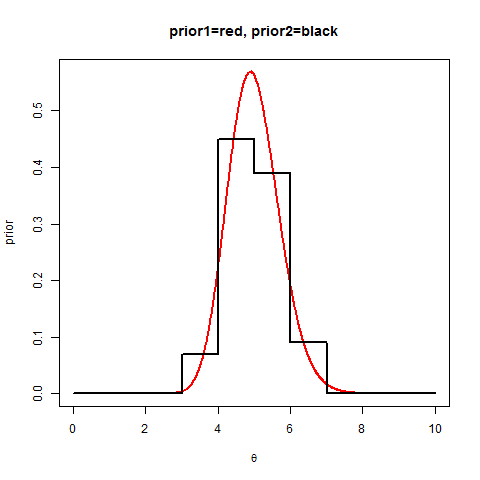
\includegraphics[scale = 0.4]{prior.png}
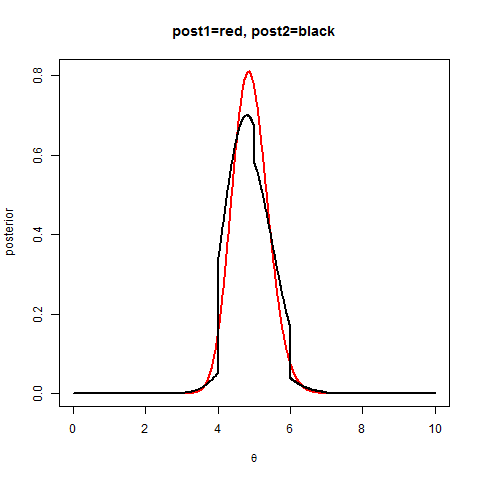
\includegraphics[scale = 0.4]{post.png}\\

\item The 95\% posterior credible interval for $p_1(\theta|y_{1:n}) $ is [3.978057, 5.916589]. The 95\% posterior credible interval for $p_2(\theta|y_{1:n}) $ is [$x_1, x_2$] where:
$$\int_{-\infty}^{x_1} p_2(\theta|y_{1:n}) = 0.025$$
$$\int_{-\infty}^{x_2} p_2(\theta|y_{1:n}) = 0.975$$
These integrals can be calculated by noting that
$$p_2(\theta|y_{1:n}) \propto \text{Gamma}(\theta|\sum y_i +1, n)$$
and simply evaluating the appropriate c.d.f.

\end{enumerate}

\pagebreak
R code:
\listinginput[1]{1}{lab8.r}

\end{document}